\section{Functional Workflow Design}
\subsection{Purpose of Sequence Model}
Sequence model diagrams show how a operation is broken down into its individual processes within the context of the relevant classes and methods. It models the explicit sequence of messages between a set of objects\cite{microsoftseq}. This allows designers and programmers at a glance to see the steps in a operation. A sequence diagram is primarily used to understand the interaction between objects, and the sequential order this occurs\cite{feliciseq}. This is useful for programmers, however it can also be for an organisations business staff, allowing individuals to communicate how the business currently works by showing how various business objects interact with each other\cite{seqbell} .

\subsection{Sequence Model Diagram of `Take Out Book'}

\begin{figure}[H]
    \centering
    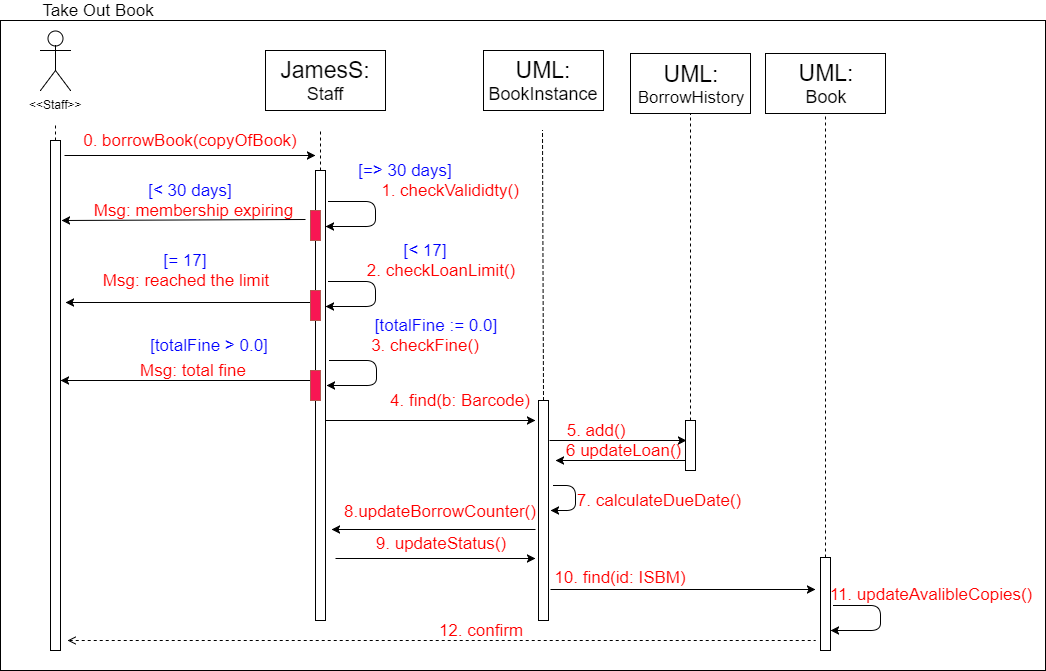
\includegraphics[width=0.9\linewidth]{image/sequence.png}
    \caption{Sequence Model Diagram}
    \label{fig:sequence}
\end{figure}

his model demonstrates how the four objects: Staff, BookInstance, BorrowHistory and Book interact with each other. It also shows the order in which they do so and the methods that they use to complete the task ‘Take Out Book’. ‘Take Out Book’ was chosen for the sequence model diagram as borrowing a book is the central feature of a library. Message 0 is the initial message that starts the sequence of events. The messages 1 to 3 deal with whether the user can validly take out a book, it checks whether they have a long enough membership, they have not yet reached their loan limit and that they do not have an outstanding loan to pay. This is done to prevent the system from allowing a user to borrow a book when they should not be able to. Message 4 finds the corresponding BookInstance according to the barcode; this is done so that the user is assigned to the correct copy of the book. In messages 5 and 6 a new BorrowHistory object is created to store details of the borrowed book in relation to the user. The process then returns to the bookInstance where message 7 calculates the due date for the book so that the user and the system knows when the book should be returned to the library. In messages 8 and 9 the borrow counter in user is updated and then the status of the bookInstance is updated. Finally in messages 10 and 11 the corresponding book class is found via its ISBN number and counter for the number of copies available is decremented. Then the process is complete and it is confirmed in message 12.

The sequence model is validated by the Use Case Diagram as the model is a representation of the Use Case ‘Take Out Book’ and also references ‘Refuse Loan’. The methods used by the sequence model diagram match the methods that are in the Class Model Diagram and the flow of events follow the outline given by the Activity Model Diagram.
